\documentclass[11pt,a4paper]{article}
\usepackage[T1]{fontenc}
\usepackage[utf8]{inputenc}
\usepackage{lmodern}
\usepackage[sc]{mathpazo}
\usepackage[scaled=.94]{helvet}
\usepackage{microtype}
\usepackage[a4paper,top=23mm,bottom=23mm,left=23mm,right=23mm,headheight=15pt]{geometry}
\usepackage{amsmath,amssymb,amsthm}
\usepackage{graphicx,xcolor,tikz}
\usetikzlibrary{arrows.meta,positioning,calc,fit,backgrounds}
\usepackage[most]{tcolorbox}
\usepackage{booktabs,tabularx,longtable,array}
\usepackage{enumitem,fancyhdr,titlesec,caption,needspace}
\usepackage{xurl}
\usepackage{hyperref,bookmark}
\definecolor{ink}{HTML}{182237}
\definecolor{night}{HTML}{111629}
\definecolor{violet}{HTML}{59439B}
\definecolor{gold}{HTML}{B48A47}
\definecolor{teal}{HTML}{276A67}
\definecolor{wine}{HTML}{7C3E54}
\definecolor{mist}{HTML}{F3F1F7}
\definecolor{sand}{HTML}{F8F5EE}
\definecolor{muted}{HTML}{526077}
\hypersetup{colorlinks=true,linkcolor=violet,citecolor=teal,urlcolor=teal,
  pdftitle={CONTINUITY OMEGA: Independently Verified Cyber Resilience},
  pdfauthor={Vincent Boucher},
  pdfsubject={Cybersecurity Resilience: Invent the Economy of Continuity},
  pdfkeywords={transformational intelligence, cyber resilience, business continuity, adversarial verification, market formation}}
\urlstyle{same}
\color{ink}
\setlength{\parindent}{0pt}
\setlength{\parskip}{6pt plus 1pt minus 1pt}
\clubpenalty=10000
\widowpenalty=10000
\displaywidowpenalty=10000
\linespread{1.055}
\setlist[itemize]{leftmargin=1.4em,itemsep=3pt,topsep=4pt}
\setlist[enumerate]{leftmargin=1.6em,itemsep=4pt,topsep=4pt}
\setcounter{tocdepth}{1}
\titleformat{\section}{\sffamily\Large\bfseries\color{violet}}{\thesection}{.65em}{}
\titleformat{\subsection}{\sffamily\large\bfseries\color{ink}}{\thesubsection}{.6em}{}
\titleformat{\subsubsection}{\sffamily\normalsize\bfseries\color{teal}}{\thesubsubsection}{.6em}{}
\titlespacing*{\section}{0pt}{16pt}{8pt}
\titlespacing*{\subsection}{0pt}{10pt}{4pt}
\pagestyle{fancy}
\fancyhf{}
\fancyhead[L]{\sffamily\small\color{muted}CONTINUITY $\Omega$}
\fancyhead[R]{\sffamily\small\color{muted}Boucher\enspace |\enspace Research edition 1.0}
\fancyfoot[L]{\sffamily\scriptsize\color{muted}TRANSFORMATIONAL INTELLIGENCE $\infty$}
\fancyfoot[R]{\sffamily\small\thepage}
\renewcommand{\headrulewidth}{.35pt}
\renewcommand{\footrulewidth}{0pt}
\captionsetup{font=small,labelfont=bf,justification=raggedright,singlelinecheck=false}
\newcolumntype{Y}{>{\raggedright\arraybackslash}X}
\newcolumntype{P}[1]{>{\raggedright\arraybackslash}p{#1}}
\renewcommand{\arraystretch}{1.2}
\newtcolorbox{insight}[1][]{enhanced,colback=mist,colframe=violet,boxrule=0pt,
  borderline west={2.4pt}{0pt}{violet},arc=0pt,left=11pt,right=11pt,top=9pt,bottom=9pt,#1}
\newtcolorbox{scopebox}[1][]{enhanced,colback=sand,colframe=gold,boxrule=.45pt,
  arc=1pt,left=10pt,right=10pt,top=8pt,bottom=8pt,#1}
\newcommand{\kicker}[1]{{\sffamily\small\bfseries\color{gold}\MakeUppercase{#1}}}
\newcommand{\om}{CONTINUITY $\Omega$}
\newcommand{\ti}{Transformational Intelligence}
\newcommand{\genesis}{ALPHA GENESIS FLYWHEEL $\Omega$}
\newcommand{\status}[1]{\textsf{\textbf{#1}}}
\newcommand{\repo}{https://github.com/MontrealAI/AGI-Alpha-Invention-Flywheel-Lab}
\newtheorem{proposition}{Proposition}
\newtheorem{definition}{Definition}
\newcommand{\chapterpage}{\clearpage}
\begin{document}
\begin{titlepage}
\thispagestyle{empty}
\begin{tikzpicture}[remember picture,overlay]
\fill[night] (current page.south west) rectangle (current page.north east);
\fill[violet!32!night] ([xshift=80mm,yshift=-58mm]current page.north west) circle (72mm);
\draw[gold!60,line width=.5pt] ([xshift=23mm,yshift=-24mm]current page.north west)--([xshift=-23mm,yshift=-24mm]current page.north east);
\draw[white!15,line width=.5pt] ([xshift=23mm,yshift=20mm]current page.south west)--([xshift=-23mm,yshift=20mm]current page.south east);
\end{tikzpicture}
\color{white}
{\sffamily\small MONTREAL.AI\enspace /\enspace QUEBEC.AI\hfill RESEARCH EDITION 1.0}\par
\vspace{26mm}
{\sffamily\fontsize{39}{44}\selectfont\bfseries CONTINUITY}\par
\vspace{2mm}
{\fontsize{90}{94}\selectfont\color{gold}$\Omega$}\par
\vspace{7mm}
{\sffamily\fontsize{25}{30}\selectfont\bfseries Keep the promise.}\par
\vspace{5mm}
{\sffamily\Large Independently verified cyber resilience}\par
\vspace{13mm}
\begin{minipage}{.90\textwidth}
\large
AI that finds the vulnerability is a breakthrough.\par
\vspace{3mm}
Intelligence that helps businesses survive the vulnerability---and invents a viable market for continuity---is a different game.
\end{minipage}
\vfill
{\sffamily\large\bfseries Cybersecurity Resilience}\par
{\sffamily\large Invent the Economy of Continuity}\par
\vspace{7mm}
{\sffamily Vincent Boucher\hfill 6 November 2026}\par
{\sffamily\small Montr\'eal, Qu\'ebec, Canada\hfill TRANSFORMATIONAL INTELLIGENCE $\infty$}\par
\vspace{9mm}
{\sffamily\footnotesize A research architecture, formal limits, reproduced synthetic evidence, and a testable first product.}
\end{titlepage}
\setcounter{page}{1}

\kicker{The paper in one minute}
\section*{The server is back. Is the business?}
\addcontentsline{toc}{section}{The paper in one minute}
A recovery dashboard can turn green while an accepted customer order has vanished. A backup supplier can exist while the production slot is already promised to someone else. A persuasive report can describe every component it considered while missing the dependency that decides whether the customer receives anything.

\begin{insight}
\large\textbf{The second intelligence asks what the first one missed.}\par
\textbf{\om\ asks what must now exist so the missing part no longer stops the business.}
\end{insight}

\textbf{The first user.} The operations director of a regional business-to-business packaging-label printer without a second production site. The owner or general manager approves commercial commitments.

\textbf{Proposed service, version one.} A controlled continuity rehearsal for one approved product: reconstruct the outstanding customer commitment, expose recovery omissions, prepare a permitted fallback production package, check the alternative provider's actual capacity and deadline, and produce a bounded Continuity Passport. The physical delivery, its independent acceptance, and payment are separate evidence stages.

\textbf{The one commercial assumption.} At least one target buyer values this independently rehearsed, reserved fallback enough to pay a price covering the complete cost, despite a credible self-service or incumbent alternative.

\textbf{The transformation.} Preserve the original customer outcome while changing the means. A business may be able to fulfill an approved order through another qualified route before its original computing and production environment is fully restored.

\textbf{The market hypothesis.} Portable, checkable production obligations plus verifiable reserved capacity may make useful continuity affordable for firms that cannot justify a duplicate facility. Each missing technical and contractual complement must actually be supplied.

\begin{scopebox}
\textbf{What this edition establishes.} A source-grounded synthesis; elementary conditional results about missing evidence, shared dependencies and capacity; and local reproduction of two existing synthetic prototypes at pinned source revisions. One has 29 tests; the other has 9 tests and a four-case competent-conventional tie. Five further probes retain a positive control, expose three verifier or inspection weaknesses, and demonstrate a known source-trust limit. Passing the original suites does not erase those counterexamples.\par
\textbf{What remains open.} Measured frontier-model advantage, authenticated real-world completeness, safe operational recovery, accepted alternate manufacturing, actual customer revenue, a repeatable market, and improved discovery across fresh successors.
\end{scopebox}

\chapterpage
\kicker{Abstract}
\section*{From a missing fact to a new ability}
\addcontentsline{toc}{section}{Abstract and contributions}
Adversarial AI critique can expose consequential omissions in a convincing answer. In cyber resilience, a missing customer obligation, shared dependency or competing capacity claim can invalidate an apparently healthy recovery. We propose \om: a research architecture for turning such omissions into constructed, testable and economically viable continuity capabilities. Its evaluation object is an authorized business commitment under declared disruption conditions. Evidence adjudicates a challenger's objection; construction changes the permitted route; separate acceptance tests the original outcome. Building on \ti, \genesis\ and \emph{Invent the Economy}, the architecture connects protected evidence, portable obligations, qualified alternative production, conserved capacity, complete costs and causal successor evaluation.

Three conditional results expose limits from indistinguishable evidence, shared prerequisites and incompatible cost/capacity thresholds. We reproduce two pinned synthetic implementations. One reconstructs two commitments totaling 1,900 units and detects three recovery discrepancies; the other ties competent conventional reconciliation on four cases. Further probes reproduce a false monetary pass, malformed-input failure and stale evidence display in the first prototype. The passing suites and counterexamples are retained together. No model-versus-model benchmark or field delivery is performed. A proposed first service and prospective experiment specify the buyer, commercial assumption, capable alternatives, separate acceptance and stop conditions. The research target is intelligence that discovers what a business promise depends on, constructs the missing means, and demonstrates both continuity and viable succession.

\textbf{Keywords:} cyber resilience; business continuity; transformational intelligence; adversarial verification; recovery semantics; complementary capabilities; market formation.

\subsection*{Contributions}
\begin{enumerate}
\item \textbf{A business-level evaluation object:} preserve and fulfill authorized commitments, including their amendments, cancellations, quality and deadlines.
\item \textbf{A constructive challenge protocol:} separate allegation, evidence, adjudication, repair, accepted delivery and qualified reuse.
\item \textbf{Explicit limits:} common evidence can conceal common omissions; backup routes can share a decisive dependency; contingent capacity cannot be promised repeatedly without a feasible activation policy.
\item \textbf{An honest evidence bridge:} reproduce existing useful engineering, challenge the checker itself, retain its conventional tie and economic failures, and specify the real experiment that could establish value.
\end{enumerate}
This is an operational synthesis and a falsifiable research programme. It does not originate adversarial critique, continuity planning, backup production, contingent contracts or independent assurance.

\chapterpage
\begingroup
\small
\setlength{\parskip}{2pt}
\tableofcontents
\endgroup
\vspace{5mm}
\begin{scopebox}
\textbf{Read by purpose.}\enspace For the product and story, read Sections~\ref{sec:promise}--\ref{sec:v1}. For the architecture and formal limits, read Sections~\ref{sec:contract}--\ref{sec:passport}. For evidence, economics and the decisive next experiment, read Sections~\ref{sec:evidence}--\ref{sec:flywheel}. The appendices give source lineage and reproduction instructions.
\end{scopebox}

\chapterpage
\section{Keep the promise}\label{sec:promise}
Suppose a language model summarizes a book. Its prose is elegant, its claims sound plausible, and the reader has not read enough of the book to assess what matters. A second model is asked to find a consequential omission. With access to the source and a clear reading purpose, it can point to the argument that changes the interpretation of everything else.

The useful result is not the second model's confidence. It is the \emph{inspectable discrepancy}: where the source says something material, how the summary fails to represent it, and why that failure matters for the reader's purpose. An omitted detail is not automatically a bad summary. A fabricated objection is not a correction. This motivating example and its materiality requirement already appear in \ti\ \cite{boucherTI}.

Now change the artifact. The first model produces a reassuring business-continuity plan. It lists backups, an alternate printer and a recovery procedure. The second model asks: \emph{Where is the accepted order that arrived after the backup? Can the alternate printer use the approved artwork without the unavailable identity service? Who has actually reserved its production slot?}

The consequential missing part is no longer a paragraph. It is an obligation or prerequisite. A company may restore what it remembers while failing the customer whose commitment it forgot.

\begin{insight}
\textbf{A recovery plan is a claim. A rehearsal is evidence. Continuity is the accepted outcome.}
\end{insight}

\subsection{The object worth constructing}
The proposed product helps a business answer an operational question: \emph{Under this declared disruption, can we still deliver this agreed result, to this customer, at this quality, by this deadline?} The answer may require fixing software. It may instead require a protected record, an interoperable production package, a permitted approval path, reserved external capacity or a different delivery sequence.

The central transformation is to separate the purpose from the inherited route. If the customer requires compliant labels on Thursday, restoring every component of Monday's infrastructure is one possible means. A qualified alternative manufacturer may be another. Neither route is admissible if it changes the required product, bypasses an approval or quietly transfers an unacceptable risk.

The architecture therefore searches over outcomes and their means together: what is worth preserving, what it depends on, what can be built, who must agree, how the result will be checked and how the whole arrangement can be funded. The consequence sought is useful activity that becomes reachable through a newly constructed arrangement. A more elaborate assurance document is valuable only if it helps establish or deliver that activity.

\section{The frontier changes the opportunity, not the burden of proof}\label{sec:frontier}
Official research reports now describe AI-assisted vulnerability discovery with executable validation. OpenAI's March 2026 Codex Security announcement describes project-specific threat modeling, vulnerability analysis, sandbox validation where possible and proposed patches \cite{codexSecurity}. Anthropic's October 2026 report describes an unreleased internal research model finding vulnerabilities and constructing five attack chains, followed by coordinated disclosure \cite{anthropicCyber}. These are provider reports about particular systems and evaluations. An unavailable internal model is not an accessible product dependency.

The opportunity for \om\ is a research inference: if models can inspect increasingly complex technical evidence, they may help identify the less visible connections between a technical failure and a business commitment. That inference requires its own evaluation. A model that finds a code defect has not thereby demonstrated that a printer can manufacture, dispatch and obtain acceptance of an order during an outage.

\subsection{What the strongest existing work already does}
Cyber resilience already addresses the ability to anticipate, withstand, recover from and adapt to adverse cyber conditions. NIST explicitly connects that engineering discipline to mission and business risk \cite{nist160}. NIST's event-recovery guidance already emphasizes realistic scenarios, playbooks, testing, metrics and lessons learned \cite{nist184}. The Canadian Centre for Cyber Security's ransomware guidance also recommends protected backups and recovery testing \cite{canadaRansomware}.

These are foundations to adopt. The proposed contribution is the attempted automation and integration of \emph{discovery, construction, evidence, voluntary exchange and reuse} around a missing continuity capability. It must improve a complete route or enable a valuable arrangement that the strongest available complete alternative cannot already supply within the same constraints.

\subsection{Why a critic needs a judge that can check}
CriticGPT provides evidence that AI criticism can assist human error finding, while documenting hallucinated criticism and limitations of the evaluated tasks \cite{criticGPT}. Debate studies find useful effects in some settings, but mixed results against direct answering across other task types \cite{kenton}. Research across many models finds substantial correlation in errors even across different providers and architectures \cite{correlated}.

The design implication is specific: model diversity is a search technique, not an independence certificate. A continuity challenger earns its keep by finding additional consequential failures at an acceptable total cost. Adjudication must be able to reject the critic as well as the original plan. A valid outcome is \emph{no consequential defect established}; another is \emph{insufficient evidence to decide}.

\chapterpage
\section{One buyer. One promise. One decisive first product.}\label{sec:v1}
\subsection{The user and the job}
The initial buyer hypothesis is an operations director at a regional B2B packaging-label printer with no second production site. This person coordinates delivery, knows the practical constraints and can specify the disrupted workflow. The owner or general manager authorizes commercial terms. The end customer supplies or confirms the relevant product acceptance requirements. A qualified alternate printer is a distinct counterparty whose participation must be obtained.

The prospective offer is a controlled rehearsal of one product and one fallback route. An example target, inherited from the existing proposed pilot, is \textbf{up to 20,000 accepted units within 48 agreed business hours} after a defined authorized activation \cite{handoffPilot}. This is a hypothesis to qualify, not capacity demonstrated by the 1,900-unit synthetic example. The calendar, time zone, start event, holidays, dispatch cutoff and partial-delivery rules must be explicit.

\subsection{What the proposed first service would do}
The presently executable portion is offline synthetic reconciliation and checking of supplied handoff constraints. The proposed operational service has five visible steps. Each presents the next decision in ordinary language.
\begin{enumerate}
\item \textbf{Choose the promise.} Identify the order family, exact output specification, acceptance authority, deadline and permitted disruption exercise.
\item \textbf{Find what recovery missed.} Reconcile the restored view against separately protected and appropriately authenticated commitment records. Display stale quantities, missing orders, improper cancellations and unresolved evidence gaps.
\item \textbf{Prepare the fallback.} Produce the minimum permitted package another qualified provider needs: current specification, rights, quantities, release authority, acceptance rules and reconciliation identifiers.
\item \textbf{Challenge the complete route.} Check current capacity, prior reservations, common dependencies, materials, quality, transport, permissions, costs and timing. Where evidence is missing, name the missing observation.
\item \textbf{Rehearse and issue the result.} Execute the authorized exercise, obtain separate acceptance and deliver a Continuity Passport stating exactly what was demonstrated, failed or remains unestablished.
\end{enumerate}
A version-one product does not need to scan an enterprise indiscriminately or claim that it prevents every attack. Its value depends on one consequential workflow reaching a defensible result. A completed document-only exercise must be labeled as such; it does not count as actual alternate manufacturing.

\subsection{The single risky commercial assumption}
\begin{insight}
\textbf{At least one target buyer values an independently rehearsed, reserved fallback for this specific commitment enough to pay a price covering its complete cost, despite a credible incumbent or self-service alternative.}
\end{insight}
Technical admissibility, data rights and a qualified provider are prerequisites. They do not answer the commercial question. A positive interview is preliminary evidence. Payment for preparation or a rehearsal establishes demand for that stage only. The stated assumption receives direct support when the buyer accepts and funds the complete qualified reservation and activation offer on terms covering its complete costs. Accepted performance, collected receipts and reconciled obligations then establish the outcome for that buyer. Repeatable market formation requires additional independent transactions, maintenance and renewals.

\section{Define the continuity contract before judging it}\label{sec:contract}
Let the authorized commitment be
\begin{equation}
\mathcal C=(O,Q,D,\mathcal S,L,A,V,X),
\end{equation}
where $O$ identifies the beneficiary outcome; $Q$ specifies quantity, quality and integrity; $D$ is the deadline and its clock; $\mathcal S$ is the declared disruption set; $L$ bounds tolerated service degradation and data loss; $A$ identifies permissions and activation authority; $V$ specifies acceptance; and $X$ lists exclusions and invalidation conditions. These are agreed task semantics, not numbers the candidate may adjust after a failure.

NIST's contingency-planning guidance supplies established concepts including business impact analysis, recovery time and recovery point objectives \cite{nist34}. \om\ uses those concepts while making the promised business outcome explicit. The time to restore a service, the age of recoverable data and the time to deliver an accepted customer outcome are different measurements.

\begin{center}\small
\begin{tabularx}{\textwidth}{P{.22\textwidth}YY}
\toprule
\textbf{Question} & \textbf{Measurement} & \textbf{What it cannot establish alone}\\
\midrule
Can the application run? & Service restored and authorized operations work. & Every accepted commitment was preserved.\\
Is the record complete? & Reconciliation against the scoped authoritative record and cutoff. & The alternative plant can fulfill it.\\
Is the fallback ready? & Compatible inputs, rights, capacity, people and transport. & The customer accepted physical output.\\
Was the promise kept? & Agreed quantity and quality accepted by deadline. & The next incident or a larger simultaneous load will succeed.\\
\bottomrule
\end{tabularx}
\end{center}

For a policy $\pi$, a particular environment $s$ and observed evidence $e$, let
\begin{equation}
\Phi(\pi,\mathcal C,s,e)=1
\end{equation}
mean that the declared acceptance predicates were met. A rehearsal establishes a scoped observation of $\Phi$, subject to the evidence's trust boundary. It does not establish $\Phi=1$ for every possible future attack. A robust model claim over $\mathcal S$ also requires that the model, dependency set and scenario coverage be justified.

The unit of evidence is therefore \emph{this commitment, this route, these conditions, these versions, this exercise}. The unit of reuse may be broader: a tested adapter, an obligation schema, a reservation procedure or a construction method. Reuse carries conditions and requalification duties, not permanent permission or universal acceptance.

\chapterpage
\section{The missing-evidence limit}\label{sec:evidenceLimit}
An adversarial reviewer cannot recover facts that no available source distinguishes. This is the precise reason to give the second model the book, rather than only the first model's summary. The business equivalent is to preserve evidence of what was promised outside the recovery view being evaluated.

\begin{proposition}[An omission can be invisible to every reviewer]
Let $h_0$ and $h_1$ be two possible histories with the same available evidence, $E(h_0)=E(h_1)$, but different truth values for a material continuity claim. Assume the reviewer's initial information and randomization supply no history-specific information beyond $E$. Any deterministic reviewer restricted to $E$ returns the same answer in both histories. Any randomized reviewer restricted to $E$, with internal randomness independent of the history, has the same output distribution in both. It therefore cannot be both sound and complete on these two histories.
\end{proposition}
\begin{proof}
The reviewer's input is identical. Its deterministic output, or its distribution conditional on internal randomness, is consequently identical. The correct claim label differs, so that output cannot correctly distinguish both histories. Adding reviewers with access only to the same evidence does not change the observation map.\end{proof}
This is a direct application of the information-limit argument in \ti\ \cite[Theorem 3.1]{boucherTI}, not a new general theorem about intelligence.

\subsection{The order that never reaches the backup}
In $h_0$, the business accepted 100 orders and restored all 100. In $h_1$, it accepted the same 100 plus an additional order after the last protected checkpoint; that additional order is absent from every available record. Both restored databases look identical. A checker that observes only those databases cannot establish whether the business has lost an accepted obligation.

An externally preserved acknowledgment, independently retained customer receipt or appropriately controlled commitment log can change the observation map. It can make the two histories distinguishable. The construction is an \emph{information channel}, not a more forceful prompt.

\subsection{Integrity is not completeness}
A hash can bind the bytes presented. A signature can bind a statement to a key under its authentication assumptions. Neither proves that the author included every obligation or told the truth. A log beside its mutable digest cannot establish independent origin. An intact prefix cannot by itself establish that no later event was accepted.

A proposed completeness instrument should bind a source identity, event range, sequence or high-water mark, acknowledgment policy, cutoff time, relevant customer scope and custody arrangement. It must address delayed records, out-of-band orders and compromised signing authority. An acknowledgment should not promise a recoverability level the record's protection cannot support. Asynchronous protection may be legitimate, but the permitted loss window and any customer-visible implication must be explicit.

\begin{scopebox}
\textbf{Abstention is information.} If available evidence is consistent with both a fulfilled and an unfulfilled commitment, the outcome is \status{NOT ESTABLISHED}. That is different from an observed \status{FAILED} exercise. It names a construction target: obtain the missing evidence, change the route so the uncertainty no longer matters, accept a separately authorized narrower claim, or stop.
\end{scopebox}

\section{From criticism to construction}\label{sec:protocol}
The proposed protocol has six stages. They are decision responsibilities, not a requirement to deploy six models or a fixed number of agents.

\begin{figure}[h!]
\centering
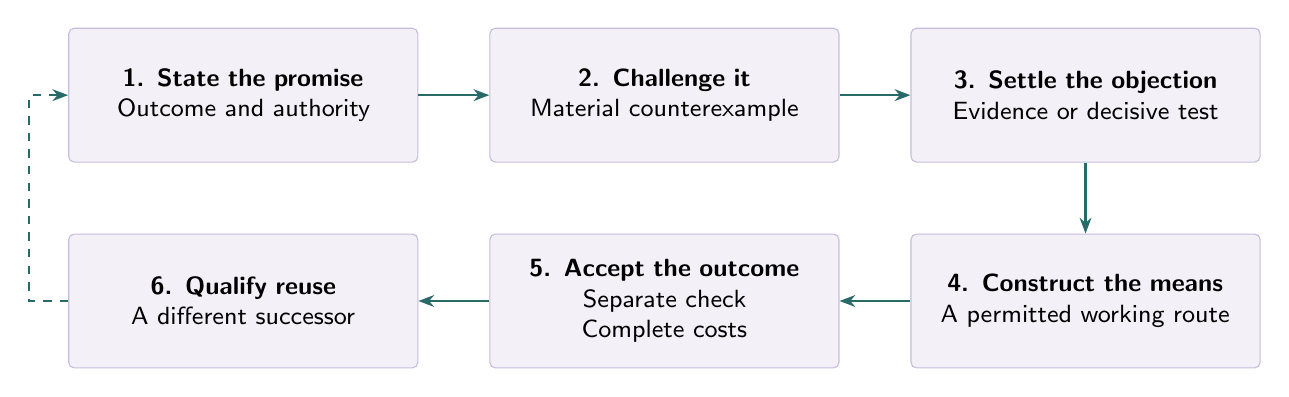
\begin{tikzpicture}[node distance=9mm and 9mm,
stage/.style={draw=violet!35,fill=mist,rounded corners=2pt,text width=42mm,minimum height=17mm,align=center,font=\sffamily\small},
arr/.style={-{Stealth[length=2mm]},thick,draw=teal}]
\node[stage] (claim) {\textbf{1. State the promise}\\Outcome and authority};
\node[stage,right=of claim] (challenge) {\textbf{2. Challenge it}\\Material counterexample};
\node[stage,right=of challenge] (test) {\textbf{3. Settle the objection}\\Evidence or decisive test};
\node[stage,below=of test] (build) {\textbf{4. Construct the means}\\A permitted working route};
\node[stage,left=of build] (accept) {\textbf{5. Accept the outcome}\\Separate check\\Complete costs};
\node[stage,left=of accept] (retain) {\textbf{6. Qualify reuse}\\A different successor};
\draw[arr] (claim)--(challenge);\draw[arr] (challenge)--(test);
\draw[arr] (test)--(build);\draw[arr] (build)--(accept);\draw[arr] (accept)--(retain);
\draw[arr,dashed] (retain.west) -- ++(-5mm,0) |- (claim.west);
\end{tikzpicture}
\caption{The challenge becomes valuable when it changes an accepted outcome or the means of a fresh successor. Every transition can also return an unresolved result or a refusal.}
\end{figure}

\subsection{Require a useful objection}
A challenge record contains the disputed claim, relevant source and version, failure mechanism, materiality, conditions of applicability, and a test or observation that could settle it. The challenger may identify a contradiction, an omitted dependency, an unavailable resource, an invalid inference or an uncertainty that prevents a responsible decision. It must be possible for the alleged failure to be refuted.

An adjudicator distinguishes an \emph{upheld objection}, a \emph{rejected objection} and an \emph{unresolved objection}. The prototype's stable handoff key binds an artifact; it is not a durable activation lock that prevents duplicate physical execution. A candidate can pass a particular check without receiving universal approval. Candidate and challenger outputs are untrusted inputs: neither may rewrite the original contract, substitute evidence or trigger privileged recovery merely by asserting that urgency requires it.

\subsection{Construct the smallest consequential change}
An upheld objection creates a specific design question. If the approved artwork is unavailable, can a separately protected current copy be prepared? If the fallback provider cannot interpret the order, can an adapter preserve its semantics? If several buyers compete for the same slot, can a truthful reservation and activation policy make the offer feasible? If restoration is too slow, can an authorized alternative route avoid the dependency?

The construction must identify what changes, what stays fixed in the customer outcome, the evidence that the new means work, their complete costs and what would invalidate them. Repairs are reevaluated against the original acceptance contract. A system cannot make a late delivery successful by changing the clock or by relabeling the customer's required quality.

\subsection{Challenge pessimism as well as optimism}
The method also challenges premature impossibility. ``We cannot recover the original plant within two days'' may be correct while ``we cannot fulfill the approved order within two days'' is false. The challenger can seek a permitted alternative production path. A found route still needs qualification; a generated alternative is neither consent nor capacity. This two-sided search is where criticism becomes useful construction rather than a catalogue of reasons to stop.

\section{Make the business obligation portable}\label{sec:portable}
Portability means preserving the information and permissions needed to satisfy the same obligation through another qualified route. It does not mean copying an entire compromised environment or transferring customer data indiscriminately.

For the printer, the minimal production package may contain the current product identifier, approved artwork version, substrate and finish, dimensional tolerances, colour reference, quantity, delivery location, deadline, lawful use rights and release authority. It also needs stable commitment identifiers, amendments, cancellations and reconciliation rules so that resumption of the primary route does not create duplicate production or invoicing.

\subsection{Three forms of continuity}
\begin{itemize}
\item \textbf{Record continuity:} preserve what was accepted and what changed, with an explicit completeness boundary.
\item \textbf{Operational continuity:} preserve or restore the means to perform the relevant work safely and correctly.
\item \textbf{Commitment continuity:} deliver the customer-valued result through an accepted route, including quality, timing and reconciliation.
\end{itemize}
These forms reinforce each other but are not equivalent. A complete log cannot manufacture labels. A functioning plant can manufacture the wrong version. A single delivered order does not establish complete enterprise recovery or the confidentiality of data exposed during the incident.

\subsection{A qualified alternative must avoid the actual failure}
Two suppliers may depend on the same identity service, substrate source, finishing equipment, release authority or transport route. Counting alternatives can conceal dependence.

\begin{proposition}[A shared prerequisite defeats nominal redundancy]
Consider all permitted routes that can meet a specified continuity contract. If every route requires prerequisite $d$, and $d$ is unavailable for the relevant interval without an admissible substitute or timely restoration, none of those routes can meet the contract in that interval.
\end{proposition}
The result follows immediately from the prerequisite relation. Its practical importance is not mathematical novelty. The difficult tasks are discovering that $d$ is shared, checking that the route set is not artificially narrow, and constructing a qualified route that avoids or restores the dependency.

\begin{insight}
\textbf{The valuable backup is an alternative path to the promised outcome.}\par
An additional machine, supplier or model helps only when the complete route remains usable under the disruption being claimed.
\end{insight}

\subsection{Secure recovery remains part of acceptance}
A route that fulfills an order by propagating a compromised artifact or using revoked credentials may fail the contract's integrity and permission requirements. The production package should have minimal disclosure, separated custody, bounded access, validated versions and a revocation path. Authorized operators must determine when affected systems and artifacts are safe to use. The exercise must also establish a separately reachable, authenticated communications and activation route for the buyer, provider and acceptance authority, with named responsibility for stopping the exercise and authorizing reconnection. The synthetic artifacts in this edition do not implement malware eradication, enterprise identity recovery or production incident response.

\section{Capacity must survive simultaneous demand}\label{sec:capacity}
A backup production slot is a scarce resource. A successful rehearsal for each buyer separately does not establish that all buyers can be served when the same incident activates their promises together. Sharing can reduce fixed costs while concentrating common-cause risk, a limitation already identified in \emph{Invent the Economy} \cite[Section 12.2]{boucherEconomy}.

Let $t$ index declared scheduling intervals. Let $q_{ij}(s,t)$ be the capacity of resource $j$ required by proposed obligation $i$ in interval $t$ under scenario $s$, in the same units as usable capacity $C_j(s,t)$. Let $a_i(s)$ indicate activation. Let $r_j(s,t)$ represent existing protected commitments not included in the proposed-obligation sum. A necessary admission condition is
\begin{equation}
\sum_i a_i(s)q_{ij}(s,t)+r_j(s,t)\leq C_j(s,t)
\quad\text{for every declared }(s,j,t).
\label{eq:capacity}
\end{equation}
It is not sufficient: setup, sequence, compatibility, materials, quality, people and transport must also fit. A final feasibility check must validate the complete schedule and contract.

\subsection{The two individually valid promises}
As an authored illustration, suppose a fallback slot can produce 2,000 acceptable units before a fixed dispatch cutoff. Two firms each reserve 1,500 units for the same activation scenario. Each promise is feasible in isolation, but the joint demand is 3,000. A truthful service must reduce admitted demand, obtain qualified additional capacity or disclose and obtain acceptance of a priority or rationing arrangement. It cannot sell both commitments as unconditional 1,500-unit coverage for that scenario.

If the product instead offers probabilistic availability, its terms must state the probability model, correlated activations, priority rules and failure consequences. An expected-load calculation does not establish a deterministic promise. Changing the product may be a legitimate newly agreed arrangement; it cannot retrospectively repair the original guarantee.

\subsection{The reservation is a maintained obligation}
A credible reservation includes resource and product scope, quantity, time window, activation conditions, existing claims, a provider acknowledgment and the consequences of expiry or withdrawal. Admission and cancellation need consistent concurrency handling: two simultaneous requests must not each observe the same free capacity and both consume it. A report that merely reads capacity cannot guarantee that another process has not reserved it before activation.

Atomic admission conserves only the reservations visible to that authority. It cannot establish that the provider disclosed every conflicting obligation or can perform. A real offer needs an evidenced reservation-book boundary, rights to verify material competing claims, observable capacity and qualification, explicit priority and failure terms, and requalification when these conditions change.

This is a proposed production requirement, not an assertion that the current synthetic handoff is a live capacity exchange. The prototype checks supplied capacity and prior reservations. It does not contact an external provider or atomically reserve its real production schedule. The paper preserves that boundary rather than upgrading a modeled Boolean into a commercial commitment.

\section{What a Continuity Passport can honestly say}\label{sec:passport}
The Passport is a compact evidence package for a particular exercised commitment. Its purpose is to help a buyer, operator and verifier reach the same bounded conclusion without trusting a model's narrative alone. It is not an insurance policy, accreditation or universal security certificate.

\begin{center}\small
\begin{tabularx}{\textwidth}{P{.25\textwidth}Y}
\toprule
\textbf{Field} & \textbf{Required meaning}\\
\midrule
Promise and authority & Beneficiary, product, quantity, quality, deadline, permissions and acceptance decision-maker.\\
Scope and conditions & Exercised disruption, environment, exclusions, known common dependencies and concurrent demand.\\
Evidence boundary & Source versions, custody, completeness cutoff, timestamps and unresolved records.\\
Working route & Current inputs, qualified production steps, reservations, transport and restoration/reconciliation procedures.\\
Observed result & What actually happened, how it was measured, contrary evidence, failures and limits.\\
Verification & Checker identity and procedure, organizational relationship, replay instructions and remaining trust assumptions.\\
Commercial state & Proposed or accepted terms; reserved or unreserved capacity; invoiced or collected payment; costs and obligations.\\
Validity & Exercise date, expiry, changes requiring recheck, revocation location and current status.\\
\bottomrule
\end{tabularx}
\end{center}

\subsection{Use explicit verdicts}
\status{DEMONSTRATED} means the stated outcome met the declared acceptance conditions in the stated exercise. \status{FAILED} means an applicable acceptance condition was violated. \status{NOT ESTABLISHED} means decisive evidence is missing, outside scope or insufficient. A Passport may demonstrate record reconciliation while leaving physical manufacturing unestablished. It should never compress all stages into a green badge.

\subsection{Specify which independence exists}
Independence has several dimensions: distinct model behavior, separate source acquisition, different checker implementation, separated execution control, independent acceptance authority and separate commercial incentives. A second agent is not automatically a second source. Separate code under common authorship is useful but can share assumptions and mistakes. An external assessor can still depend on incomplete supplied records. Each dimension should be disclosed rather than aggregated into an unsupported score.

For this paper, separately tasked AI agents reviewed the synthesis, sources and prototype evidence. They operated within one assistant workflow. This is not a benchmark of two independently selected frontier models and not third-party certification. The prototype checker implementations are inspectable; their real-world authority, source completeness and operational independence remain separate questions.

\subsection{Make evidence expire when the claim changes}
A changed artwork version, signing authority, product process, production slot, customer acceptance rule or material supplier can invalidate part of the evidence. Dependencies determine the recheck. The record of an old exercise remains true as history, while its applicability to a new promise may expire. This distinction prevents both permanent false assurance and unnecessary repetition of every unchanged check.

\section{Existing executable evidence, reproduced without relabeling}\label{sec:evidence}
This edition builds on existing repository work. It does not create another financial authority, modify the two prototypes or replace their owning branches. Local reproductions use the exact public source revisions identified below. They establish execution of the specified synthetic checks in this environment; they do not establish operational adoption of those branches or the current release status of unrelated work.

\subsection{Prototype A: reconstruct and challenge the handoff}
The source for repository PR~278 at revision \texttt{a755d0375693} supplies a synthetic label-printer example and a separate checker \cite{handoffSource}. Its event history contains three original orders, an amendment and a cancellation. Replaying the supplied history leaves \textbf{two outstanding commitments totaling 1,900 units}.

The recovered snapshot has three discrepancies: a stale quantity, a missing accepted order and a cancelled order still present. The producer constructs a fallback package; the checker independently replays the supplied events and validates the resulting obligations and modeled constraints. The source's test suite contains \textbf{29 tests}. The reproduction also runs all 12 supplied CLI cases: three pass the synthetic handoff check and nine correctly refuse it before handoff. Separate CLI verification of the nominal artifacts passes. A handoff pass does not repair or validate the malformed restored snapshot; it checks the separately reconstructed fallback package. These tests are implementation checks over authored data, not 29 customers, outages or independent trials of an AI system.

The supplied provider has 3,200 units of nominal capacity and 1,100 already reserved, leaving 2,100. The 1,900-unit package fits that modeled availability. The stipulated lead time is 22 hours against a 48-hour requirement. Those are fixture values: execution time of the Python program does not measure manufacturing or outage duration.

The same authored example uses a US\$5,700 quote and US\$5,050 of modeled full cost, giving US\$650 of modeled contribution, below a hypothetical buyer cap of US\$5,800. These are not observed market prices or actual receipts. External acquisition, implementation, model, host, verification and liability costs require measurement in a real campaign; a fixture's complete-cost fields do not establish completeness of actual economics.

\subsection{Prototype B: a strong conventional control ties}
The source for draft PR~277 at revision \texttt{84c4288b4726} checks commitments across a synthetic recovery \cite{recoverySource}. Its \textbf{9 tests} include missing obligations, altered evidence and replay-related checks. Its authored four-case decision vector is \texttt{[PASS, FAIL, FAIL, FAIL]}: a healthy case passes, while the three supplied defective cases fail.

A competent conventional reconciliation route returns the same vector in all four cases. A health-only route accepts defective cases, but that weak route is not the relevant basis for an AI-superiority claim. The conventional tie is a result worth preserving: business-semantic verification matters; this comparison does not show that the proposed method uniquely supplies it.

\begin{center}\small
\begin{tabularx}{\textwidth}{P{.25\textwidth}YY}
\toprule
\textbf{Evidence} & \textbf{Supported conclusion} & \textbf{Unsupported extension}\\
\midrule
29 handoff tests & The supplied cases exercise reconciliation and modeled handoff constraints. & Real provider readiness or actual cyber resilience.\\
9 recovery tests & The supplied recovery checker rejects specific faulty records and claims. & Measured frontier-model discovery skill.\\
Four-case control tie & Competent conventional reconciliation matches these case decisions. & General inferiority or superiority in all workflows.\\
1,900-unit fixture & The authored outstanding obligations reconcile to that quantity. & 20,000-unit physical delivery capacity.\\
\bottomrule
\end{tabularx}
\end{center}

\subsection{Challenge the checker, too}\label{sec:checkerChallenge}
A passing test suite can itself become a reassuring but incomplete summary. A later repository hardening review reported input and evidence-display weaknesses in the pinned handoff source \cite{handoffHardening}. We independently reran five compact probes against the unchanged \texttt{a755d0375693} bytes. These are targeted engineering counterexamples, separate from the 29-test suite and not a sample estimating real-world failure rates.

\begin{center}\small
\begin{tabularx}{\textwidth}{P{.24\textwidth}YY}
\toprule
\textbf{Probe} & \textbf{Observed result} & \textbf{What it means}\\
\midrule
Nominal positive control & The original synthetic handoff passes. & The probe setup preserves the intended baseline.\\
Boolean monetary offer & A coherently adjusted zero-cost case passes when its offer is JSON \texttt{true}; the constructor rejects that value. & The verifier does not independently enforce the constructor's monetary type rule.\\
Malformed top-level case & Calling the audit with \texttt{None} raises \texttt{AttributeError}. & This input receives an exception, not a structured refusal.\\
Changed handoff after audit & \texttt{inspect} returns the old readiness Passport; fresh \texttt{verify} exits 3 with \status{FAIL}. & Reading a stored status does not re-establish the current artifact's validity.\\
Coherently rewritten source & A resealed amendment changes the total from 1,900 to 2,000 units and passes. & Internal consistency cannot authenticate the supplied scenario; this was an already-disclosed trust boundary.\\
\bottomrule
\end{tabularx}
\end{center}

The source bytes remain unchanged. The companion preserves the probe construction, observations and replay command. It does not qualify the later proposed repair or silently substitute that repair's test count. The result is narrower and more useful: the original suites pass, and the original checker still has demonstrated weaknesses. Production acceptance needs independent shape and type validation, a protected scenario reference, and fresh checking of the artifacts actually presented. Even a matching external digest establishes equality to its reference, not the reference's truth or completeness.

\begin{insight}
\textbf{The verifier is part of the claim. It must also survive a challenge.}
\end{insight}

\subsection{The earlier economic failure remains a failure}
The prior GENESIS Commitment~001 simulation reports a central buyer refusing an offer that only ties its authored outside option, with a modeled loss of US\$1,080 \cite{genesisResults}. Favorable scenarios in that work depend on different authored assumptions. This paper does not pool those scenarios, reinterpret their simulation as paid demand or use them to fund a new enterprise. The negative case is directly relevant: a useful recovery construction can still fail to justify purchase.

\subsection{What the reproduction does not test}
The histories, capacities, consent flags, costs and recovery times are supplied fixtures. Local hash consistency does not authenticate their origin or completeness. The runs do not inject a cyberattack, restore a real plant, manufacture labels, obtain external acceptance or collect payment. No model API is called by the reproduced prototypes. The study therefore cannot estimate how often frontier models find novel omissions, how much their errors correlate here or whether they outperform capable human and AI alternatives.

\chapterpage
\section{Invent the economy of continuity}\label{sec:economy}
The economic unit is the complete arrangement. An alternate printer with spare machinery, a customer worried about downtime and an excellent verification script do not automatically form a market. The product must connect usable capability, willing counterparties, enforceable operational commitments, acceptance and feasible cash timing \cite{boucherEconomy}.

\subsection{Who contributes, who decides, who pays}
\begin{center}\small
\begin{tabularx}{\textwidth}{P{.21\textwidth}YY}
\toprule
\textbf{Participant} & \textbf{Contribution} & \textbf{Reason to participate, to be tested}\\
\midrule
Buyer business & Requirements, permitted records, activation and payment. & A credible improvement over its complete outside option.\\
Fallback provider & Qualified capacity, personnel, process and delivery. & Reservation and production compensation cover obligations and opportunity cost.\\
Verifier & Independent evidence checks and scoped acceptance record. & A fee for competent assessment, without a reward for issuing a pass.\\
Integrator & Preparation, coordination, maintained interfaces and rehearsal. & Collected receipts cover the entire service and its residual duties.\\
End customer & Product acceptance and necessary permissions. & Continuity preserves the promised value without unacceptable substitution.\\
\bottomrule
\end{tabularx}
\end{center}
Some roles may be combined if their conflicts and trust assumptions are disclosed. More organizations do not automatically mean better assurance. The arrangement should be as simple as the outcome permits.

\subsection{A price window is a condition, not a sales forecast}
Let $p$ be payment to the service coalition, and let $B$ be the buyer's justified maximum payment after its own implementation burden and best complete outside option are considered. Let $C$ be the coalition's complete economic cost and obligations for the same scope and horizon, including construction, failed attempts, acquisition, data preparation, reservation, rehearsal, production, transport, verification, maintenance, financing and retained obligations, with no double counting. A nonnegative-contribution price can exist only if
\begin{equation}
C\leq p\leq B.
\end{equation}
Positive contribution requires a strict margin after the relevant costs. Neither $B$ nor actual $C$ is established by a model inventing values for them. Customer preference can depend on trust, disruption burden, quality, contractual risk and the continuing ability to self-provide. A complex offer may lose even when its spreadsheet appears attractive.

\subsection{Complementarity can change feasibility}
Let $x\in\{0,1\}$ indicate a qualified portable production package, and $y\in\{0,1\}$ indicate a compatible reserved-capacity arrangement. Define $F(x,y)$ to mean that the complete offer satisfies the contract, voluntary participation, capacity and cash constraints.

The diagnostic pattern $F(0,0)=F(1,0)=F(0,1)=0$ and $F(1,1)=1$ identifies joint sufficiency within the supplied model: neither intervention alone closes the stated gap. It is an experimental contrast to test, not a new theorem.
This is a conditional complementarity statement, not proof that these conditions hold in a market. It becomes useful when the failed predicates are named: perhaps reserved capacity is unusable without approved specifications, while portable specifications have no value during simultaneous demand without a reserved slot. A competent conventional provider must be allowed to construct both. If a competent provider already supplies the same outcome on equally acceptable terms at equal or lower full cost, this comparison establishes no incremental advantage for the proposed construction. The offer may still be viable, and the conventional route should be used when it is the best complete means.

\subsection{Pooling must pass both the cost and the capacity test}
Sharing preparation costs can make an offer cheaper while making its promises mutually incompatible. Consider a deliberately simple fixed-period model. There are $n$ equal buyers; each requires $q>0$ units if the declared common disruption occurs. All can activate together. Available compatible capacity after prior claims is $C\geq0$. Common qualification and reservation cost is $K>0$; additional worst-case cost is $c\geq0$ per buyer. Each pays one fee $p\leq B$, where $B>c$ is a supplied willingness-to-pay ceiling. There are no additional activation receipts. All relevant period costs are assumed included, and cash timing is checked separately.

\begin{proposition}[A feasible pool needs an overlap]
Under this model, a buyer count supporting both nonnegative contribution and all admitted activations exists if and only if
\begin{equation}
\left\lceil\frac{K}{B-c}\right\rceil
\leq
\left\lfloor\frac{C}{q}\right\rfloor.
\label{eq:pool}
\end{equation}
This statement allows the supplied ceiling fee $p=B$ and assumes every integer buyer count in the interval is available and willing under the model. Positive contribution additionally requires $n(B-c)>K$.
\end{proposition}
\begin{proof}
For any admissible fee, contribution is at most $n(B-c)-K$, so nonnegative contribution requires $n\geq\lceil K/(B-c)\rceil$. Simultaneous activation requires $nq\leq C$, hence $n\leq\lfloor C/q\rfloor$. These are necessary. If the interval contains an integer $n$, choosing $p=B$ satisfies both inequalities under the stated assumptions.\end{proof}

\textbf{Authored illustration.} Let $K=900$, $c=100$ and $B=400$ in hypothetical monetary units, with $C=2{,}000$ capacity units and $q=750$ per buyer. Economics needs at least three buyers; capacity permits at most two. Two buyers leave a 300-unit monetary shortfall. Three buyers reach break-even but promise 2,250 capacity units. No pool works under these assumptions. More customers do not repair it.

The missing means might reduce common qualification cost, obtain genuinely independent capacity, change the production process or support a separately accepted service design. Added capacity has its own reservation and delivery costs. Changing those inputs requires a new evaluated arrangement. Equation~\eqref{eq:pool} is a transparent application of shared-cost economics and capacity conservation, not a market forecast or a production scheduler.

\subsection{Cash must arrive before the action it funds}
Let $K_0$ be authorized opening cash allocated to this arrangement, before deducting protected amounts. Let $I_{\leq t}$ be collected inflows and $O_{\leq t}$ cash outflows through a proposed action prefix $t$. Let $R_t$ be cash that must remain protected for reserves and obligations not already discharged in those outflows. After including each proposed outlay, financeability requires
\begin{equation}
K_0+I_{\leq t}-O_{\leq t}-R_t\geq 0.
\end{equation}
The condition applies to each relevant funding and failure path. Paid obligations must not remain in $R_t$, and forecast receipts cannot enter collected inflows. A profitable expected contract may fail this condition if capacity and rehearsal must be paid for before the buyer pays. Forecast receipts are not cash. Financing requires actual accepted terms and supported accounting; it is not revenue or earned surplus. This paper specifies constraints and creates no new ledger, account or authority.

\subsection{A practical proposed offer}
A first offer can price an authorized scoped rehearsal and preparation service, followed only after qualification by a separately accepted reservation and activation arrangement. Fees should correspond to delivered preparation, maintained availability and accepted production, with explicit cancellation, rework and refund treatment. The staged offer reduces the cost of learning, but acceptance of an earlier paid stage must not be reported as acceptance of the full continuity arrangement. The verifier should not be paid more for a favorable verdict. Insurance, if later involved, is a separately underwritten relationship; the Passport does not itself grant coverage or predict a premium.

The arrangement should remain useful when AI makes preparation cheaper. Charging for an increasing number of critiques would reward avoidable work. Compensation should follow useful outcomes and actual obligations. A smaller price or fewer repeated checks can be progress if the service remains sustainable and the customer benefits.

\section{The experiment that could earn the claim}\label{sec:experiment}
The next decisive step is one authorized real rehearsal with an actual target buyer and a qualified provider, compared with a competent complete alternative. It should be designed before results are observed. The experiment can establish a narrow case, while leaving broad market and model claims open. Before prospecting, register eligible targets, outreach method, recruitment window, campaign budget and required accepted price and payment conditions. No qualifying purchase within those conditions rejects this offer-campaign; it does not establish that no continuity market can exist.

\subsection{Freeze the promise and the evidence boundary}
Before execution, specify the original order and acceptance, the disruption and its safe exercise procedure, the protected source record, external custody and completeness policy, product rights, provider capacity and competing reservations, transport deadlines, costs, cash stages and permissible interventions. Agree on what counts as a production drill, a substitute test or a tabletop exercise. Preserve failed runs and material changes.

The study needs a clean separation between acceptance of a rehearsal and acceptance of a manufactured delivery. If the buyer permits only a non-production substitute, report that result. No software test can silently supply the physical observation it was not authorized to make.

\subsection{Compare capable complete alternatives}
For the programme's productivity question, the primary control is competent human professionals using conventional software, without frontier-model assistance. Conventional software retains its real automation and speed. Fully autonomous and hybrid AI operations are reported separately, with actual internal human intervention and costs disclosed. This human-only control measures the chosen labor-productivity question. Incremental transformational-value claims require comparison with the strongest permitted complete AI-assisted or autonomous alternative.

For the commercial decision, additional complete alternatives include the current provider, a human-plus-AI service, a strong single model with tools, other autonomous services, self-provision and no purchase. Give the proposed system and controls equivalent records, permissions, capacity opportunities, acceptance and total resource budgets. Do not reserve the better supplier or richer source evidence for the proposed arm.

\subsection{Separate finding, building and selling}
\begin{enumerate}
\item \textbf{Find the blocker.} Use blinded eligible cases and source access to measure consequential omissions found, false allegations, unresolved cases and total review cost. Compare a critic workflow with matched-cost additional direct reasoning and conventional reconciliation.
\item \textbf{Close the blocker.} Give every arm the same adjudicated counterexample. Compare complete routes to accepted output. This prevents better initial information from being mislabeled as better construction.
\item \textbf{Make it viable.} Measure technical portability alone, capacity/contract changes alone and their joint construction as explanatory ablations. Then compare the joint route with the strongest unrestricted complete alternative. Obtain actual voluntary acceptance and account for collected money and all campaign costs.
\end{enumerate}
The limited ablations diagnose complementarity. They are not the primary competitor and cannot establish superiority by denying the baseline a useful intervention.

\subsection{Measure outcomes that matter}
Primary measures include accepted correct commitments delivered by deadline; missing, duplicate or incorrect units; unsupported continuity claims accepted; valid critical omissions detected; correct abstentions; unnecessary refusals; and actual complete cost per accepted result. Record elapsed time, customer friction, operator effort, privacy/permission failures, rework, refunds and continuing liabilities. Count all attempted eligible cases, not only successful demonstrations.

The critical failure test is a false continuity assurance: a claimed success when an applicable original commitment fails. Measure it separately from false alarms. A system that rejects everything has a low false-assurance rate but no useful continuity service.

\subsection{Decision and stop rules}
Do not proceed to a stronger claim if the completeness required by the scoped contract cannot be established, permissions are absent, the provider cannot substantiate its current capacity, output acceptance fails or the proposed arrangement cannot meet its cash and obligation constraints. If the capable alternative delivers the same outcome at lower complete cost, use it. If no real buyer accepts at a sustainable price, retain the useful engineering and record that the offer has not earned a commercial claim.

A single success supports this exercised case. Additional buyers, providers, order families and disruption conditions are required before inferring repeatability. Sample size and statistical analysis should follow a stated effect, baseline variance and error costs; this paper does not invent empirical rates to manufacture a power calculation.

\chapterpage
\section{The flywheel: keep what makes a different promise possible}\label{sec:flywheel}
\genesis\ separates seeing a frontier capability, discovering its useful consequences and improving the machinery that discovers those consequences \cite{boucherGenesis}. \om\ supplies a specific candidate path through those three functions.

\textbf{Proposed first turn.} A paid and accepted rehearsal identifies a missing dependency, constructs a qualified portable obligation package and validates a fallback. It retains the usable adapter, failure conditions, verification procedure and measured costs. Any unrestricted collected earnings remain distinct from reserves, liabilities and forecast income.

\textbf{Proposed different successor.} A genuinely different obligation class or workflow requires a new construction: for example, a different production process with different prerequisites and acceptance requirements. A second buyer purchasing substantially the same offering tests repeatability; it does not by itself establish a new enabling opportunity. The retained package may reduce specification transfer, reconciliation or qualification costs. It may also be incompatible, stale or more expensive to adapt than a conventional new solution. Either result is informative.

\textbf{Potential next opportunity.} If the transfer works and counterparties accept it, several qualified providers might offer standardized, non-conflicting continuity slots to smaller firms. Another successor might be interoperability for emergency procurement rather than another printer. These are proposed opportunities, not established new markets.

\subsection{Three tests prevent a decorative flywheel}
\begin{enumerate}
\item \textbf{Financed by earnings.} Did collected unrestricted surplus from the first accepted activity actually pay the successor's costs while prior obligations remained protected?
\item \textbf{Enabled by the retained capability.} Under matched starting resources, does removing that capability make the successor less feasible or more costly than the strongest route without it? Ordinary equal-content reuse is a required comparison.
\item \textbf{A better discovery process.} With initial tools and information held comparable, does the changed discovery procedure perform better across fresh independently selected campaigns after acquisition and verification costs?
\end{enumerate}
These tests answer different questions. A successor can be funded by earnings even when the original capital could also have funded it. Better tools can improve production without improving invention. A later task is not evidence that the earlier task enabled it.

\begin{insight}
\textbf{The durable asset is not the argument between the agents.}\par
It is the qualified capability, the conditions under which it works, and---when separately demonstrated---a better way to construct the next one.
\end{insight}

Retain compact, useful failure lessons as well as successes: an untrusted cutoff, a shared substrate dependency, a verifier that accepted a forged package or a buyer who rationally declined. Preserve essential source and financial evidence; retire redundant transcripts and obsolete machinery. Learning should improve the next decision, not merely expand the archive.

\chapterpage
\section{Failure modes the architecture must face}\label{sec:failures}
\begin{longtable}{P{.25\textwidth}P{.68\textwidth}}
\toprule
\textbf{Failure mode} & \textbf{Required response and remaining limit}\\
\midrule
\endhead
Shared model blind spot & Use original sources, distinct checks and incremental-failure measurement. Different providers still may share errors.\\
Invented criticism & Require materiality and a reproducible basis; adjudicate against positive controls as well as failures. Critic confidence is not evidence.\\
Incomplete source universe & Establish a scoped external completeness boundary or abstain. A well-formed digest cannot prove absent events do not exist.\\
Compromised authority & Check key and approval custody, revocation and permitted activation. A valid signature under a compromised key does not restore trust.\\
Common dependency & Examine full supplier and service paths, including material and transport dependencies. Scenario coverage remains bounded.\\
Overbooked standby & Check aggregate conditional obligations and concurrent admission, not only isolated buyer exercises. The live provider must actually reserve.\\
Late or unsuitable output & Test final quality and delivery acceptance. Boot time, dispatch time and customer receipt are distinct.\\
Biased acceptance & Separate production and acceptance control and disclose assessor relationships. Organizational independence still needs competent evidence.\\
Stale Passport & Bind dependencies, versions and time windows; invalidate affected claims when they change. Historical evidence stays historical.\\
Financially infeasible rescue & Count prefunding, failures, refunds and protected obligations. Expected positive contribution is not available cash.\\
Unwanted product & Compare complete outside options and observe voluntary purchase. Technical correctness cannot compel demand.\\
Unsupported generalization & Preserve the precise tested scope. Local synthetic success cannot certify a field operation or all future attacks.\\
\bottomrule
\end{longtable}

\subsection{Security of the intelligence workflow}
Documents, logs and tool outputs may contain malicious instructions. They are evidence to inspect, not authority to change the task. The challenger should operate with the minimum required access, and any executable tests should run in a specifically authorized isolated environment. Data minimization, controlled secrets, separated signing and acceptance, and a reversible recovery path belong in the implementation design. The paper and local reproductions do not demonstrate those controls in a production deployment.

\subsection{Limits of the research contribution}
The formal observations are elementary and conditional. The prototypes use authored cases. The manuscript's AI review shares one workflow and is not independent institutional assessment. No new comparative frontier-model performance, live recovery, physical-production result, real price, collected revenue or successor advantage is claimed. The thesis can fail: capable existing services may already provide the complete offer; the missing evidence may be unobtainable; correlated demand may make reservation too costly; or buyers may rationally prefer self-service.

These are decisive possibilities to investigate. They do not require abandoning the useful purpose. They require changing or retiring an inadequate means while preserving what the evidence actually established.

\section{Conclusion: the economy of keeping promises}
Finding a vulnerability can reveal how a system may fail. Continuity asks what useful activity can still be delivered when that failure matters. Transformational intelligence makes the route itself editable: the record, the information channel, the production process, the verification method, the participants and the arrangement that makes their cooperation worthwhile.

The strongest version of adversarial AI is constructive. It does not end with one model defeating another in an argument. It produces an objection that can be checked, a missing means that can be built, an outcome that someone can accept and a cost that the enterprise can actually bear.

\om\ proposes a concrete first step: one business, one customer commitment, one qualified fallback, one authorized disruption and one independently adjudicated result. The existing synthetic prototypes make parts of that path executable. The handoff checker's counterexamples, the recovery checker's conventional tie and the earlier GENESIS simulation's modeled commercial failure identify exactly what the next test must resolve.

If that test succeeds, the reusable result may help a different business preserve a different promise. If collected surplus finances that next step, the enterprise has a funded continuation. If a retained construction method improves fresh discovery under capable controls, the flywheel has earned a deeper claim. Each link requires its own evidence.

\begin{insight}
\large\textbf{Find what the plan missed.}\par
\textbf{Build what keeping the promise requires.}\par
\textbf{Prove the result within its scope.}\par
\textbf{Use what survives to make the next promise possible.}
\end{insight}

\chapterpage
\appendix
\section{Source lineage and what this paper adds}\label{app:lineage}
The three supplied research papers are treated as distinct foundations, with their original assumptions and evidence intact. Public editions are linked in the references. Printed page numbers below are used; \genesis\ v2 has a cover, so its printed page is one less than its PDF page.

\begin{longtable}{P{.28\textwidth}P{.24\textwidth}P{.40\textwidth}}
\toprule
\textbf{Foundation} & \textbf{Relevant passage} & \textbf{Application here}\\
\midrule
\endhead
\ti & p.~1; Appendix C, pp.~22--23 & The summary example; source-grounded materiality; a criticism is not automatically correct.\\
\ti & p.~3; Theorem 3.1, p.~4 & Purpose/formulation/evaluator separation; the missing-evidence limit.\\
\ti & pp.~7--8, 10--12 & Executable transformation, evidence-preserving production, strong comparisons and separately authorized evaluation.\\
\emph{Invent the Economy} & p.~3; Theorem 3.1, p.~5 & Technical capability and voluntary arrangement as one construction; separate evidence stages and complementarity.\\
\emph{Invent the Economy} & pp.~9--10, 17 & Prefunding and successor constraints; obstructions as construction targets; shared failures and genuine independence.\\
\genesis\ v2 & pp.~6--8 & Frontier awareness, consequence discovery and improved machinery as separate claims; jointly enabling means.\\
\genesis\ v2 & pp.~12--13, 16--18 & Full costs, customer alternatives, native cash, conventional ties and limits of simulated operation.\\
\bottomrule
\end{longtable}

\textbf{Specific synthesis.} This paper specializes those foundations to preservation and fulfillment of customer commitments during cyber disruption. It connects external evidence completeness, portable obligation semantics, common dependencies, simultaneous capacity claims, a revocable evidence package, a specific first buyer and a prospective commercial test.

\textbf{Relationship to earlier critique research in the repository.} \emph{SURF THE EXPONENTIAL---The Missing Move} already develops constructive criticism and reusable means \cite{boucherSurf}. The present paper is a distinct application to continuity, with its own scope, source identities and evidence record. Its test counts are not added to or substituted for that earlier paper's studies.

\chapterpage
\section{Reproduction and evidence identity}\label{app:reproduction}
The companion stores a compact reproduction record, source identities, a claim register and build instructions. The prototype source remains at its original pinned public revisions; this paper does not vendor a duplicate implementation. Check the listed Git blob identities before interpreting a reproduction.

\begin{scopebox}
\textbf{Handoff source, PR 278:}\par
\texttt{a755d0375693465f8f31c0c919cc186eae74bbcc}\par
\textbf{Recovery source, PR 277:}\par
\texttt{84c4288b4726a17a90f8462d1d6faf8b5f8f00b5}\par
\textbf{Initial main revision inspected:}\par
\texttt{48be73cd1259b9c212431b0fa1594a6c87698372}
\end{scopebox}
The source revision is the scientific identity. PR descriptions and later branch heads can change. These reproductions are fresh isolated synthetic runs, not migration or resumption of any existing financial account. No private checkpoint, signing authority or customer record is part of the publication.

For the handoff source, run the following in a clean checkout of the first revision, using a new output directory. The backslash joins the first command across lines:
\begin{quote}\small\ttfamily
python3 -m unittest discover -s tests \textbackslash{}\par
\hspace*{1em}-p 'test\_continuity\_omega.py' -v\par
python3 -m continuity\_omega demo --out /tmp/continuity-NEW\par
python3 -m continuity\_omega verify --in-dir /tmp/continuity-NEW
\end{quote}
For the recovery source, run its test file and the demonstration command documented in its pinned README. The companion reproduction report records the actual commands, exit results, case vector and source hashes. The 29- and 9-test suites are separate, hand-authored engineering checks. Combining them does not create a statistical sample or an empirical AI benchmark.

The companion's \texttt{counterexamples.py} separately reproduces the five probes in Section~\ref{sec:checkerChallenge} against the same pinned handoff source. Its success means the stated weaknesses and control observations were reproduced; it does not mean that the checker passed a production qualification. The compact record is \texttt{evidence/COUNTEREXAMPLES.json}.

The manuscript compiles with a standard TeX Live installation and no shell escape. The publication manifest identifies the canonical PDF bytes. A rebuild on a different TeX distribution may produce different metadata or PDF bytes; compare the textual content and source, and preserve the canonical checksum. Checksums establish file identity, not the truth of the claims.

\chapterpage
\section{A minimum useful exercise record}\label{app:record}
For a real pilot, the following record is proposed. It is an operational specification requiring actual counterparties and permissions, not an executed agreement.
\begin{enumerate}
\item \textbf{Promise:} order identifier, beneficiary, specification, quantity, quality, delivery deadline and acceptance authority.
\item \textbf{Disruption:} exercised failure, activation event, permitted actions, isolation and stop procedure.
\item \textbf{Evidence:} external source custody, completeness interval, acknowledgments, version binding, unresolved out-of-band obligations and missing records.
\item \textbf{Alternative:} provider, approved inputs, materials, permissions, responsible personnel, capacity interval, other reservations, shared dependencies and transport.
\item \textbf{Challenge:} exact allegation, source reference, why it matters, proposed discriminating check and adjudication.
\item \textbf{Execution:} actual observations, elapsed times, errors, failed attempts, corrections, operator intervention and controlled deviations.
\item \textbf{Acceptance:} who checked what, with which independence, and what the customer actually accepted.
\item \textbf{Economics:} collected payments, all costs, financing, refunds, liabilities, reserved capacity and remaining duties.
\item \textbf{Passport:} separate verdicts for reconciliation, readiness, physical delivery and commercial outcome; exclusions, expiry and revocation.
\item \textbf{Successor:} retained asset, applicability, new task, strongest complete comparator, equal-content reuse and all requalification costs.
\end{enumerate}

\subsection*{Review and disclosure}
The manuscript was prepared with AI assistance and separate task-based critiques within one assistant workflow. The review challenged unsupported independence, source completeness, aggregate capacity, physical acceptance, commercial inference and successor causality. The companion records the resulting corrections and remaining limits. This process is manuscript quality control, not external peer review, certification or evidence of a two-frontier-model performance advantage.

\chapterpage
\begingroup
\setlength{\parskip}{2pt}
\begin{thebibliography}{99}
\footnotesize
\setlength{\itemsep}{3pt}
\bibitem{boucherTI} Vincent Boucher. \emph{Transformational Intelligence: Learning to Change the Game}. Research manuscript, October 2026. \url{https://montrealai.github.io/AGI-Alpha-Invention-Flywheel-Lab/transformational-intelligence.html}.
\bibitem{boucherGenesis} Vincent Boucher. \emph{ALPHA GENESIS FLYWHEEL $\Omega$: Riding the Exponential---Three Orders of Intelligence for an Enterprise That Discovers What Becomes Possible}. Research edition 2.0, 4 November 2026. \url{https://montrealai.github.io/AGI-Alpha-Invention-Flywheel-Lab/alpha-genesis-flywheel-omega-v2.html}.
\bibitem{boucherEconomy} Vincent Boucher. \emph{Invent the Economy: Transformational Intelligence for Creating Viable Markets}. Research manuscript, October 2026. \url{https://montrealai.github.io/AGI-Alpha-Invention-Flywheel-Lab/invent-the-economy.html}.
\bibitem{codexSecurity} OpenAI. \emph{Codex Security: now in research preview}. 6 March 2026. Provider report. \url{https://openai.com/index/codex-security-now-in-research-preview/}.
\bibitem{anthropicCyber} Nicholas Carlini, David Dworken, Xinyang Ge, Ben Morris, Milad Nasr, Chris Rohlf, and Luna Tong. \emph{Discovering and exploiting vulnerabilities in critical, real-world software with Claude}. Anthropic, 27 October 2026. Provider report. \url{https://www.anthropic.com/research/discovering-vulnerabilities-with-claude}.
\bibitem{criticGPT} OpenAI. \emph{Finding GPT-4's mistakes with GPT-4}. 27 June 2024. \url{https://openai.com/index/finding-gpt4s-mistakes-with-gpt-4/}.
\bibitem{kenton} Zachary Kenton et al. \emph{On scalable oversight with weak LLMs judging strong LLMs}. arXiv:2407.04622, 2024. \url{https://doi.org/10.48550/arXiv.2407.04622}.
\bibitem{correlated} Elliot Kim, Avi Garg, Kenny Peng, and Nikhil Garg. \emph{Correlated Errors in Large Language Models}. ICML 2025; arXiv:2506.07962. \url{https://doi.org/10.48550/arXiv.2506.07962}.
\bibitem{nist160} Ron Ross, Victoria Pillitteri, Richard Graubart, Deborah Bodeau, and Rosalie McQuaid. \emph{Developing Cyber-Resilient Systems: A Systems Security Engineering Approach}. NIST SP 800-160 Vol.~2 Rev.~1, December 2021. \url{https://doi.org/10.6028/NIST.SP.800-160v2r1}.
\bibitem{nist184} Michael Bartock, Jeffrey Cichonski, Murugiah Souppaya, Matthew Smith, Gregory Witte, and Karen Scarfone. \emph{Guide for Cybersecurity Event Recovery}. NIST SP 800-184, December 2016. \url{https://doi.org/10.6028/NIST.SP.800-184}.
\bibitem{nist34} Marianne Swanson, Pauline Bowen, Amy Wohl Phillips, Dean Gallup, and David Lynes. \emph{Contingency Planning Guide for Federal Information Systems}. NIST SP 800-34 Rev.~1, updated 11 November 2010. \url{https://doi.org/10.6028/NIST.SP.800-34r1}.
\bibitem{canadaRansomware} Canadian Centre for Cyber Security. \emph{Ransomware playbook (ITSM.00.099)}. Second release, 28 January 2026. \url{https://www.cyber.gc.ca/en/guidance/ransomware-playbook-itsm00099}.
\bibitem{handoffSource} MONTREAL.AI. \emph{CONTINUITY $\Omega$: synthetic commitment handoff prototype}. Public source at \texttt{a755d0375693}, inspected and reproduced 6 November 2026. \url{https://github.com/MontrealAI/AGI-Alpha-Invention-Flywheel-Lab/tree/a755d0375693465f8f31c0c919cc186eae74bbcc/continuity_omega}.
\bibitem{handoffPilot} MONTREAL.AI. \emph{CONTINUITY $\Omega$: First paid-pilot acceptance contract}. Proposed specification, no real approvals; source at \texttt{a755d0375693}. \url{https://github.com/MontrealAI/AGI-Alpha-Invention-Flywheel-Lab/blob/a755d0375693465f8f31c0c919cc186eae74bbcc/docs/continuity-omega/REAL_PILOT.md}.
\bibitem{recoverySource} MONTREAL.AI. \emph{CONTINUITY $\Omega$: verify obligations across recovery}. Public research source at \texttt{84c4288b4726}, inspected and reproduced 6 November 2026. \url{https://github.com/MontrealAI/AGI-Alpha-Invention-Flywheel-Lab/tree/84c4288b4726a17a90f8462d1d6faf8b5f8f00b5/campaign/continuity_omega_20261106}.
\bibitem{genesisResults} MONTREAL.AI. \emph{GENESIS Commitment 001: results, costs and adjudication}. Historical simulation at \texttt{607c18854db0}. \url{https://github.com/MontrealAI/AGI-Alpha-Invention-Flywheel-Lab/blob/607c18854db04dc3aa4adf242a4e3d1d9c629880/campaign/genesis_commitment001/RESULTS.md}.
\bibitem{boucherSurf} Vincent Boucher. \emph{SURF THE EXPONENTIAL---The Missing Move}. Research edition 1.2.0, 6 November 2026. \url{https://montrealai.github.io/AGI-Alpha-Invention-Flywheel-Lab/surf-the-exponential.html}.
\bibitem{handoffHardening} MONTREAL.AI. \emph{CONTINUITY $\Omega$ 0.2: reproduced failures and evidence-boundary hardening}. Proposed source at \texttt{6cd7e1bb7197}, inspected 6 November 2026; not qualified by this paper. \url{https://github.com/MontrealAI/AGI-Alpha-Invention-Flywheel-Lab/blob/6cd7e1bb7197cabdf8f3d093eead662cde5351f4/docs/continuity-omega/HARDENING.md}.
\end{thebibliography}
\endgroup
\end{document}
